Con el fin de obtener mejores resultados, las estructuras cristalinas 
utilizadas en las simulaciones pasaron por un proceso de relajaci\'on. 
Para los cuales se definieron los siguientes limites de convergencia: 
$10^{-5}$eV para la variaci\'on m\'axima de energ\'ia, $0,03eV$\AA$^{-1}$ 
para la fuerza y $0,05$ Gp para la presi\'on. Este proceso de relajaci\'on se 
realiz\'o para cada arreglo antiferromagn\'etico de cada material utilizado. 
Cada valor mostrado en las gr\'aficas siguientes, es el resultado de un 
c\'alculo de campo autoconsistente en el cual se var\'ian los par\'ametros de 
red, se calcula la energ\'ia total y la fuerza sobre la estructura cristalina. 
Estos pasos de c\'alculo de campo autoconsistente se iteran siendo las 
condiciones iniciales de cada paso las condiciones finales del paso anterior, 
hasta converger con las restricciones antes mencionadas.

\noindent El proceso de relajaci\'on entrega un archivo de texto extenso, que 
contiene 
muchos pasos intermedios de la simulaci\'on junto a los datos de inter\'es. Por 
ello es necesario realizar un procesamiento de este archivo para extraer los 
datos importantes y poder realizar las gr\'aficas de energ\'ia total vs 
iteraci\'on y las gr\'aficas de fuerza vs iteraci\'on. El procesamiento del 
archivo se realiz\'o con un script shell.

\subsection{$\mathbf{BiFeO_{3}}$ con arreglo antiferromagn\'etico tipo A}

\begin{table}[H]
    \begin{center}
        \caption{Comparaci\'on entre los par\'ametros de red antes y despu\'es 
        de la relajaci\'on del $BiFeO_{3}$ con arreglo antiferromagn\'etico 
        tipo A.}
        \begin{tabular}{ccc}
            \hline
               & \textbf{Inicial} \cite{tomar2018} & \textbf{Final} \\
            \hline \hline
            a (\AA) & $5.57$  & $5.65$   \\
            \hline
            c (\AA) & $13.86$ & $14.16$   \\
            \hline
        \end{tabular}
        \singlespace
        \label{bfo_a_ini_fin}
    \end{center}
\end{table}

\noindent La tabla \ref{bfo_a_ini_fin} muestra la comparaci\'on entre los 
par\'ametros de red del $BiFeO_{3}$ con arreglo antiferromagn\'etico tipo A 
antes y despu\'es de la relajaci\'on.

\begin{figure}[H]
    \centering
    \subfloat[]{
        \label{bfo_fuerza_a}
        
        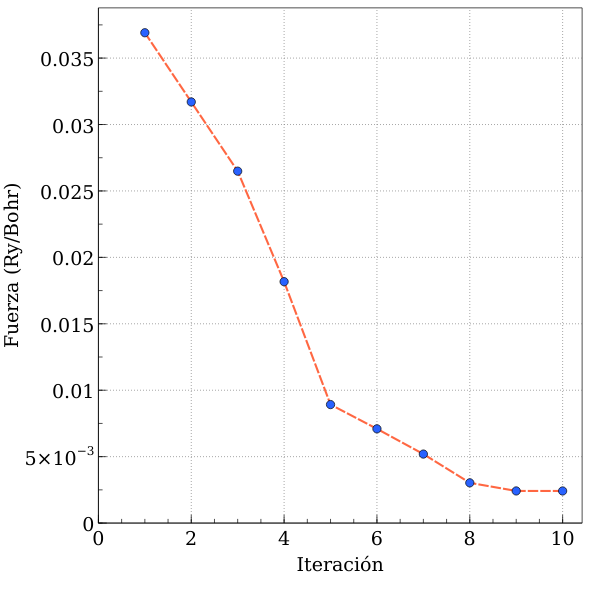
\includegraphics[width=0.5\textwidth]{contenido/resultados/relajacion/img_relajacion/fuerza_BFO_A.png}}
    \subfloat[]{
        \label{bfo_energia_a}
        
        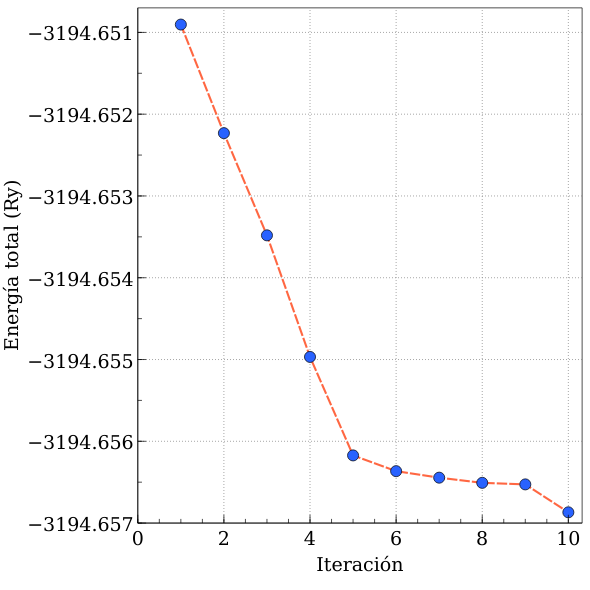
\includegraphics[width=0.5\textwidth]{contenido/resultados/relajacion/img_relajacion/energia_BFO_A.png}}
    \singlespace
    \caption[Minimizaci\'on de la fuerza y la energ\'ia del $BiFeO_{3}$ con 
    arreglo antiferromagn\'etico tipo 
    A]{\ref{minimizacion_bfo_A} \subref{bfo_fuerza_a} Minimizaci\'on de la 
    fuerza sobre la estructura antiferromagn\'etica de tipo A del $BiFeO_{3}$. 
    \ref{minimizacion_bfo_A} \subref{bfo_energia_a} Minimizaci\'on de la 
    energ\'ia de la estructura antiferromagn\'etica de tipo A del $BiFeO_{3}$.}
    \label{minimizacion_bfo_A}
\end{figure}

\noindent La figura \ref{minimizacion_bfo_A} muestra la minimizaci\'on de la 
fuerza \ref{minimizacion_bfo_A} \subref{bfo_fuerza_a} y de la energ\'ia 
\ref{minimizacion_bfo_A} \subref{bfo_energia_a} del $BiFeO_{3}$ con arreglo 
antiferromagn\'etico tipo A. Se puede observar que el sistema converge luego de 
10 iteraciones.

\subsection{$\mathbf{BiFeO_{3}}$ con arreglo antiferromagn\'etico tipo G}

\begin{table}[H]
    \begin{center}
        \caption{Comparaci\'on entre los par\'ametros de red antes y despu\'es 
            de la relajaci\'on del $BiFeO_{3}$ con arreglo antiferromagn\'etico 
            tipo G.}
        \begin{tabular}{ccc}
            \hline
            & \textbf{Inicial} \cite{tomar2018} & \textbf{Final} \\
            \hline \hline
            a (\AA) & $5.57$  & $5.64$   \\
            \hline
            c (\AA) & $13.86$ & $14.07$   \\
            \hline
        \end{tabular}
        \singlespace
        \label{bfo_g_ini_fin}
    \end{center}
\end{table}

\noindent La tabla \ref{bfo_g_ini_fin} muestra la comparaci\'on entre los 
par\'ametros de red del $BiFeO_{3}$ con arreglo antiferromagn\'etico tipo G 
antes y despu\'es de la relajaci\'on.

\begin{figure}[H]
    \centering
    \subfloat[]{
        \label{bfo_fuerza_g}
        
        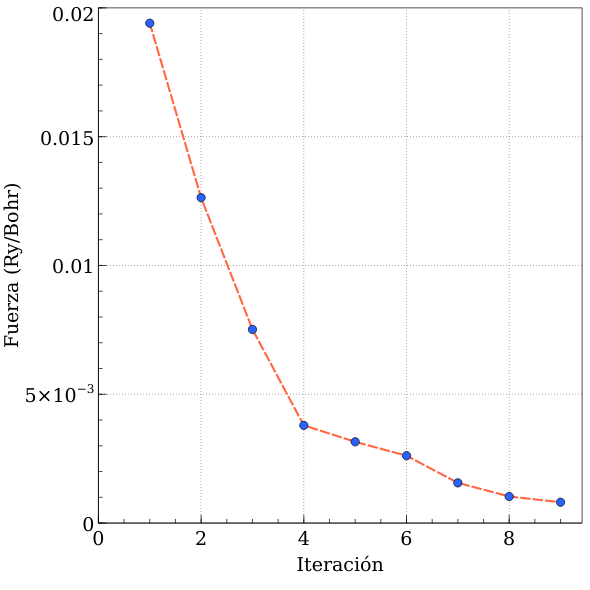
\includegraphics[width=0.5\textwidth]{contenido/resultados/relajacion/img_relajacion/fuerza_BFO_G.png}}
    \subfloat[]{
        \label{bfo_energia_g}
        
        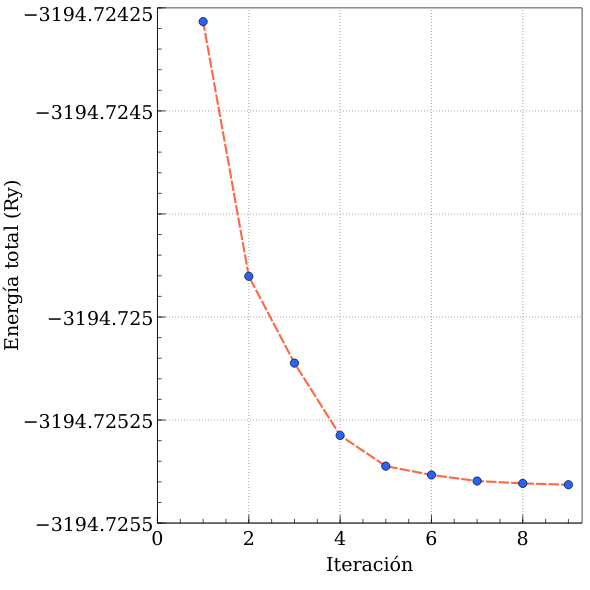
\includegraphics[width=0.5\textwidth]{contenido/resultados/relajacion/img_relajacion/energia_BFO_G.png}}
    \singlespace
    \caption[Minimizaci\'on de la fuerza y la energ\'ia del $BiFeO_{3}$ con 
    arreglo antiferromagn\'etico tipo 
    G]{\ref{minimizacion_bfo_G} \subref{bfo_fuerza_g} Minimizaci\'on de la 
        fuerza sobre la estructura antiferromagn\'etica de tipo G del 
        $BiFeO_{3}$. 
        \ref{minimizacion_bfo_G} \subref{bfo_energia_g} Minimizaci\'on de la 
        energ\'ia de la estructura antiferromagn\'etica de tipo G del 
        $BiFeO_{3}$.}
    \label{minimizacion_bfo_G}
\end{figure}

\noindent La figura \ref{minimizacion_bfo_G} muestra la minimizaci\'on de la 
fuerza \ref{minimizacion_bfo_G} \subref{bfo_fuerza_g} y de la energ\'ia 
\ref{minimizacion_bfo_G} \subref{bfo_energia_g} del $BiFeO_{3}$ con arreglo 
antiferromagn\'etico tipo G. Se puede observar que el sistema converge luego de 
9 iteraciones.

\subsection{$\mathbf{YCrO_{3}}$ con arreglo antiferromagn\'etico tipo A}

\begin{table}[H]
    \begin{center}
        \caption{Comparaci\'on entre los par\'ametros de red antes y despu\'es 
            de la relajaci\'on del $YCrO_{3}$ con arreglo antiferromagn\'etico 
            tipo A.}
        \begin{tabular}{ccc}
            \hline
            & \textbf{Inicial} \cite{geller1956} & \textbf{Final} \\
            \hline \hline
            a (\AA) & $5.247$  & $5.14$   \\
            \hline
            b (\AA) & $5.518$ & $5.49$   \\
            \hline
            c (\AA) & $7.54$ & $7.41$   \\
            \hline
        \end{tabular}
        \singlespace
        \label{yco_a_ini_fin}
    \end{center}
\end{table}

\noindent La tabla \ref{yco_a_ini_fin} muestra la comparaci\'on entre los 
par\'ametros de red del $YCrO_{3}$ con arreglo antiferromagn\'etico tipo A 
antes y despu\'es de la relajaci\'on.

\begin{figure}[H]
    \centering
    \subfloat[]{
        \label{yco_fuerza_a}
        
        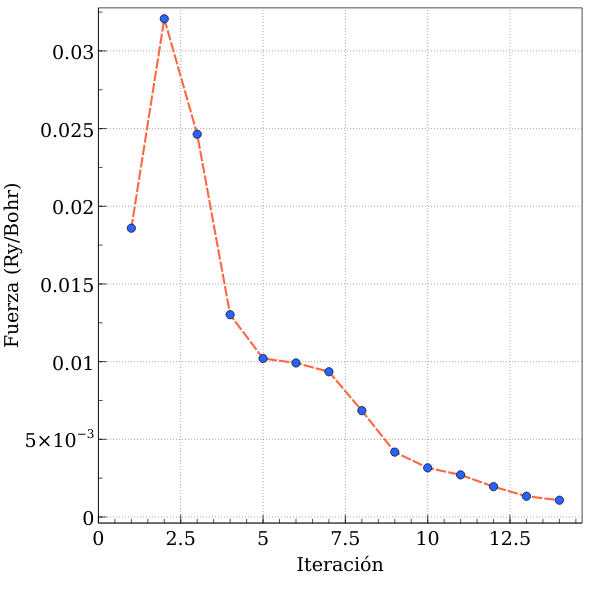
\includegraphics[width=0.5\textwidth]{contenido/resultados/relajacion/img_relajacion/fuerza_YCO_A.png}}
    \subfloat[]{
        \label{yco_energia_a}
        
        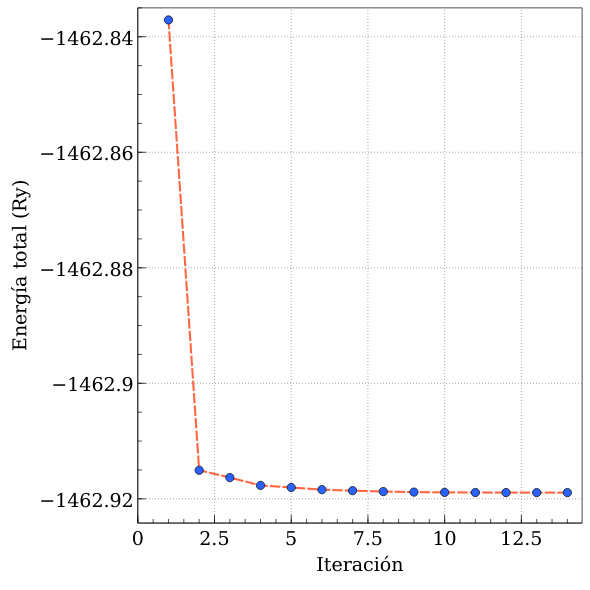
\includegraphics[width=0.5\textwidth]{contenido/resultados/relajacion/img_relajacion/energia_YCO_A.png}}
    \singlespace
    \caption[Minimizaci\'on de la fuerza y la energ\'ia del $YCrO_{3}$ con 
    arreglo antiferromagn\'etico tipo 
    A]{\ref{minimizacion_yco_A} \subref{yco_fuerza_a} Minimizaci\'on de la 
        fuerza sobre la estructura antiferromagn\'etica de tipo A del 
        $YCrO_{3}$. 
        \ref{minimizacion_yco_A} \subref{yco_energia_a} Minimizaci\'on de la 
        energ\'ia de la estructura antiferromagn\'etica de tipo A del 
        $YCrO_{3}$.}
    \label{minimizacion_yco_A}
\end{figure}

\noindent La figura \ref{minimizacion_yco_A} muestra la minimizaci\'on de la 
fuerza \ref{minimizacion_yco_A} \subref{yco_fuerza_a} y de la energ\'ia 
\ref{minimizacion_yco_A} \subref{yco_energia_a} del $YCrO_{3}$ con arreglo 
antiferromagn\'etico tipo A. Se puede observar que el sistema converge luego de 
14 iteraciones.


\subsection{$\mathbf{YCrO_{3}}$ con arreglo antiferromagn\'etico tipo C}

\begin{table}[H]
    \begin{center}
        \caption{Comparaci\'on entre los par\'ametros de red antes y despu\'es 
            de la relajaci\'on del $YCrO_{3}$ con arreglo antiferromagn\'etico 
            tipo C.}
        \begin{tabular}{ccc}
            \hline
            & \textbf{Inicial} \cite{geller1956} & \textbf{Final} \\
            \hline \hline
            a (\AA) & $5.247$  & $5.15$   \\
            \hline
            b (\AA) & $5.518$ & $5.47$   \\
            \hline
            c (\AA) & $7.54$ & $7.42$   \\
            \hline
        \end{tabular}
        \singlespace
        \label{yco_c_ini_fin}
    \end{center}
\end{table}

\noindent La tabla \ref{yco_c_ini_fin} muestra la comparaci\'on entre los 
par\'ametros de red del $YCrO_{3}$ con arreglo antiferromagn\'etico tipo C 
antes y despu\'es de la relajaci\'on.

\begin{figure}[H]
    \centering
    \subfloat[]{
        \label{yco_fuerza_c}
        
        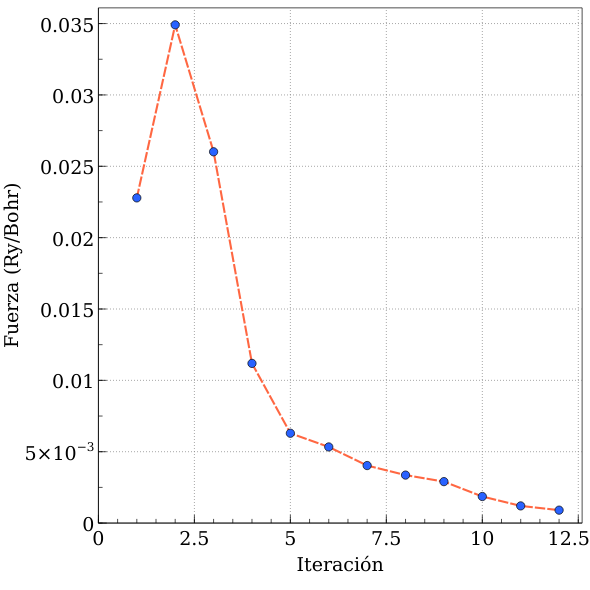
\includegraphics[width=0.5\textwidth]{contenido/resultados/relajacion/img_relajacion/fuerza_YCO_C.png}}
    \subfloat[]{
        \label{yco_energia_c}
        
        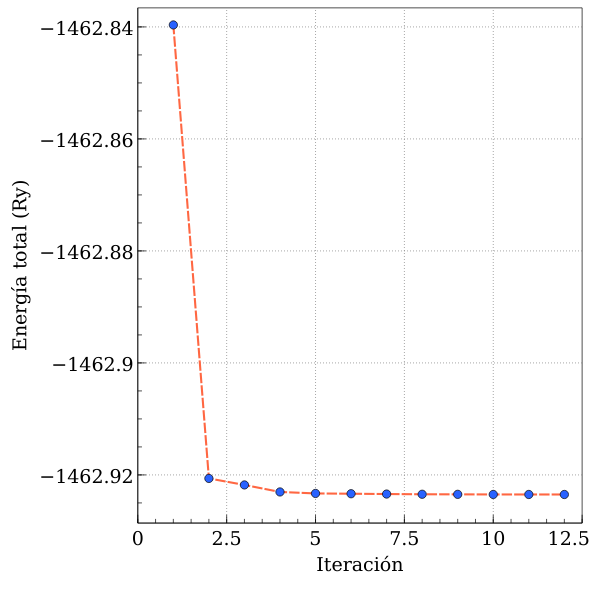
\includegraphics[width=0.5\textwidth]{contenido/resultados/relajacion/img_relajacion/energia_YCO_C.png}}
    \singlespace
    \caption[Minimizaci\'on de la fuerza y la energ\'ia del $YCrO_{3}$ con 
    arreglo antiferromagn\'etico tipo 
    C]{\ref{minimizacion_yco_C} \subref{yco_fuerza_c} Minimizaci\'on de la 
        fuerza sobre la estructura antiferromagn\'etica de tipo C del 
        $YCrO_{3}$. 
        \ref{minimizacion_yco_C} \subref{yco_energia_c} Minimizaci\'on de la 
        energ\'ia de la estructura antiferromagn\'etica de tipo C del 
        $YCrO_{3}$.}
    \label{minimizacion_yco_C}
\end{figure}

\noindent La figura \ref{minimizacion_yco_C} muestra la minimizaci\'on de la 
fuerza \ref{minimizacion_yco_C} \subref{yco_fuerza_c} y de la energ\'ia 
\ref{minimizacion_yco_C} \subref{yco_energia_c} del $YCrO_{3}$ con arreglo 
antiferromagn\'etico tipo C. Se puede observar que el sistema converge luego de 
12 iteraciones.


\subsection{$\mathbf{YCrO_{3}}$ con arreglo antiferromagn\'etico tipo G}

\begin{table}[H]
    \begin{center}
        \caption{Comparaci\'on entre los par\'ametros de red antes y despu\'es 
            de la relajaci\'on del $YCrO_{3}$ con arreglo antiferromagn\'etico 
            tipo G.}
        \begin{tabular}{ccc}
            \hline
            & \textbf{Inicial} \cite{geller1956} & \textbf{Final} \\
            \hline \hline
            a (\AA) & $5.247$  & $5.14$   \\
            \hline
            b (\AA) & $5.518$ & $5.47$   \\
            \hline
            c (\AA) & $7.54$ & $7.41$   \\
            \hline
        \end{tabular}
        \singlespace
        \label{yco_g_ini_fin}
    \end{center}
\end{table}

\noindent La tabla \ref{yco_g_ini_fin} muestra la comparaci\'on entre los 
par\'ametros de red del $YCrO_{3}$ con arreglo antiferromagn\'etico tipo G 
antes y despu\'es de la relajaci\'on.

\begin{figure}[H]
    \centering
    \subfloat[]{
        \label{yco_fuerza_g}
        
        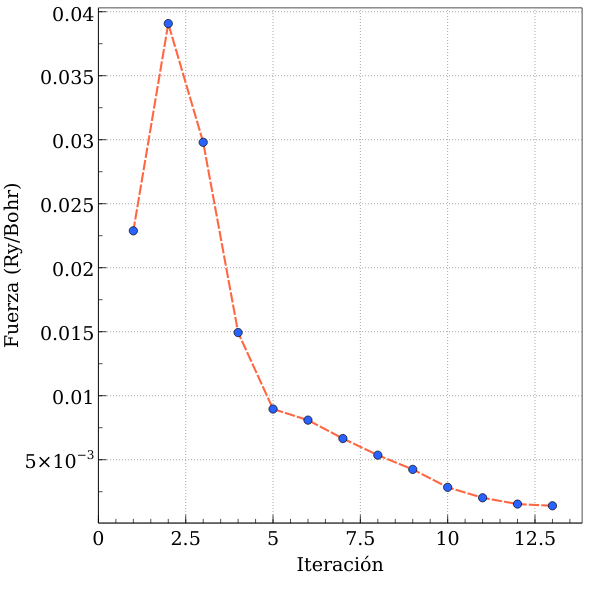
\includegraphics[width=0.5\textwidth]{contenido/resultados/relajacion/img_relajacion/fuerza_YCO_G.png}}
    \subfloat[]{
        \label{yco_energia_g}
        
        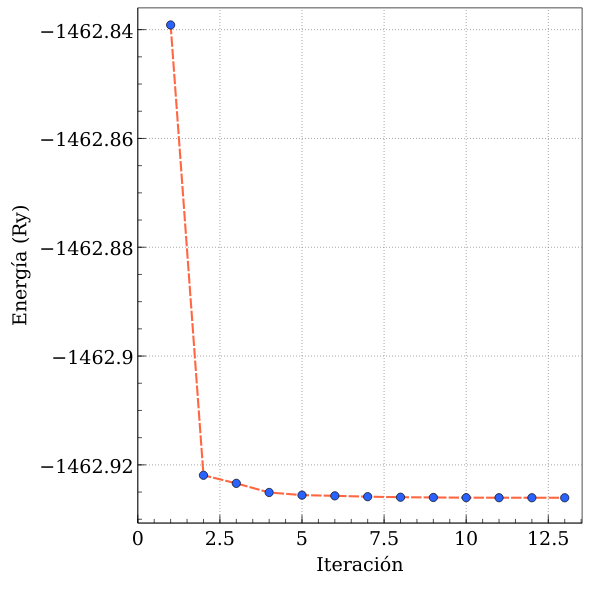
\includegraphics[width=0.5\textwidth]{contenido/resultados/relajacion/img_relajacion/energia_YCO_G.png}}
    \singlespace
    \caption[Minimizaci\'on de la fuerza y la energ\'ia del $YCrO_{3}$ con 
    arreglo antiferromagn\'etico tipo 
    G]{\ref{minimizacion_yco_G} \subref{yco_fuerza_g} Minimizaci\'on de la 
        fuerza sobre la estructura antiferromagn\'etica de tipo G del 
        $YCrO_{3}$. 
        \ref{minimizacion_yco_G} \subref{yco_energia_g} Minimizaci\'on de la 
        energ\'ia de la estructura antiferromagn\'etica de tipo G del 
        $YCrO_{3}$.}
    \label{minimizacion_yco_G}
\end{figure}

\noindent La figura \ref{minimizacion_yco_G} muestra la minimizaci\'on de la 
fuerza \ref{minimizacion_yco_G} \subref{yco_fuerza_g} y de la energ\'ia 
\ref{minimizacion_yco_G} \subref{yco_energia_g} del $YCrO_{3}$ con arreglo 
antiferromagn\'etico tipo G. Se puede observar que el sistema converge luego de 
13 iteraciones.
